\documentclass{article}

\usepackage{amsmath, amssymb}			%For typesetting mathematical symbols and the such
\usepackage{moreverb}				%Enable verbatim environment
\usepackage[dvips]{graphicx}			%For graphics to load nicely
\usepackage[margin=2.5cm]{geometry}		%Nice way of changing the margins
\pagestyle{myheadings}				%Change headers
\markright{Vincent Quenneville-Belair}

\begin{document}

%%%%%%%%%%%%%%%%%%%%%%%%%%%%%%%%%%%%%%%%%%%%%%%%%%%%%%%%%%%%%%%%%%%%

\begin{center}
\large Sample Lab Report 2\\
\large Vincent Quenneville-Belair
\end{center}

\section*{Preliminaries}

Notice that you can put many     spaces                  in between words, and LaTeX ignores them. 
If you want to start a new paragraph you need to skip a line in the code.
Otherwise, the lines will be in the same paragraph.

In LaTeX, round parenthesis don't mean anything (since we use them in text too often!). Instead, command parameters are passed using \emph{curly} brackets. 

Begin commands start new environment. For instance, the align environment is used to enter math.
The \& allows to align stuff in equation
Remember: LaTeX is very flexible with respect to spacing. If you want to start a new line, you need to type two backslashes.
\begin{align}
2\theta_t 
&= 2\arcsin{\frac{\lambda}{2d}} \\
&= \int_a^{\infty}f(x)dx.
\end{align}
Here's an inline equation $2\cos\theta_t$, and then an example of a matrix, while also removing the equations numbering (by adding a * next to the environment name).
Remember: the spacing is very flexible.
\begin{align*} 
	\begin{pmatrix} 
		1 & 2 \\ 
		3 & 4 
	\end{pmatrix}
= \begin{bmatrix} 1 & 2 \\ 0 & 0 \end{bmatrix} + \begin{bmatrix} 0 & 0 \\ 3 & 4 \end{bmatrix}.
\end{align*}
Let's now show how to include this pretty graph.
\begin{center}
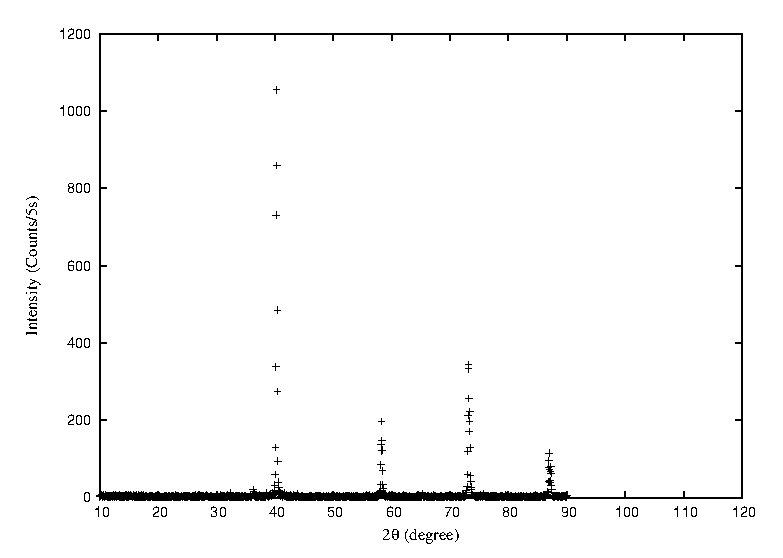
\includegraphics[width=6cm]{example.eps} 
\end{center}

%%%%%%%%%%%%%%%%%%%%%%%%%%%%%%%%%%%%%%%%%%%%%%%%%%%%%%%%%%%%%%%%%%%%

\section*{Exercise 1}

Inputting the augmented matrix for the given system of equations.
\begin{verbatim}
format rational
A=[2 -1 4 -5 27; -1 3 -2 -1 -26; 0 1 5 -6 15; 3 -8 1 0 53]
\end{verbatim}
MatLab can spit out LaTeX code for matrices by using latex(A) or, sometimes, latex(sym(A)).
\begin{align*}
 \left[ \begin {array}{ccccc} 2&-1&4&-5&27\\\noalign{\medskip}-1&3&-2&-1&-26\\\noalign{\medskip}0&1&5&-6&15\\\noalign{\medskip}3&-8&1&0&53\end {array} \right] 
\end{align*}

Getting the augmented matrix into row echelon form by doing row operations.
\begin{verbatim}
A(1,:)=A(1,:)+A(2,:);
A(2,:)=A(2,:)+A(1,:);
A(4,:)=A(4,:)-3*A(1,:);
A([2 3],:)=A([3 2],:);
A(3,:)=A(3,:)-5*A(2,:);
A(4,:)=A(4,:)+14*A(2,:);
A(3,:)=A(3,:)+A(4,:);
A(4,:)=A(4,:)-A(3,:);
A(3,:)=A(3,:)-A(4,:);
A(4,:)=A(4,:)-A(3,:);
A(3,:)=A(3,:)-A(4,:);
A(4,:)=A(4,:)-A(3,:);
A(4,:)=A(4,:)-A(3,:);
A(3,:)=A(3,:)/5;
A(4,:)=A(4,:)/31;
\end{verbatim}
The row echelon form of the initial augmented matrix
\begin{align*}
 \left[ \begin {array}{ccccc} 1&2&2&-6&1\\\noalign{\medskip}0&1&5&-6&15\\\noalign{\medskip}0&0&1&-{\frac {17}{5}}&4\\\noalign{\medskip}0&0&0&1&0\end {array} \right] 
\end{align*}
 
Solving the system by back-substitution.
From last row we get $x_4 = 0$.
From 3rd row, $x_3 - \frac{17}{5}x_4 = 4$, so $x_3 = 4$.
From 2nd row, $x_2 + 5x_3 -6x_4 = 15$, hence $x_2 = -5$.
From 1st row, $x_1 + 2x_2 + 2x_3 - 6x_4 = 1$, so $x_1 = 3$.

Solution: $x_1 = 3, x_2 = -5, x_3 = 4, x_4 = 0$.

%%%%%%%%%%%%%%%%%%%%%%%%%%%%%%%%%%%%%%%%%%%%%%%%%%%%%%%%%%%%%%%%%%%%

\section*{Exercise 2}

Row operations to get the augmented matrix in row echelon form
\begin{verbatim}
A=[-2 1 9 1; 3 3 -4 2; 1 4 5 5];
A([1 3],:)=A([3 1],:);
A(2,:)=A(2,:)-3*A(1,:), A(3,:)=A(3,:)+2*A(1,:);
A(2,:)=A(2,:)+A(3,:);
\end{verbatim}
so $A$ is
\begin{align*}
\left[ \begin {array}{cccc} 1&4&5&5\\\noalign{\medskip}0&0&0&-2\\\noalign{\medskip}0&9&19&11\end {array} \right] 
\end{align*}
Clearly the system does not have a solution, since the second row implies $0x_1 + 0x_2 + 0x_3 = 0 = -2$, a contradiction.

\end{document}
